\chapter{Requirements}
\label{chapter:requirements}

\section{Overview}

The foundation for this project was laid during the requirements gathering and formulation phase. In order to deliver a good system and streamline the planning process, one first has to develop a strong understanding of the tasks a B\&B system has to fulfil as well as the challenges that it should overcome. Further, as exemplified by Boehm \cite{Boehm1988} and Brooks \cite{Brooks1975}, incorrect and incomplete requirements can lead to an exponential increase in cost during later stages of project development. For these reasons, a considerable amount of the early project phase was spent on gathering requirements, as can be seen in figure \ref{gantt-chart}.

The requirements were gathered in an iterative process, starting with collective brainstorming during the team's weekly group meetings. Most of the team members had used online accommodation booking solutions before and could thus derive initial requirements from their own prior experiences. Next, the team studied current online accommodation booking services and took note of the functionality they offered. This research resulted in an exhaustive initial requirements list. Most of the essential requirements were so-called CRUD (Create, Read, Update, Delete) operations that each concerned a different entity in the System. These categories were therefore used to structure the requirements list seen below. Through subsequent iteration, especially during the use case definition phase, the initially long requirements list was condensed into a concise set of project requirements. Importance was assigned to the requirements according to the MoSCoW scale, ranking them based on their importance: whether they \textbf{M}ust, \textbf{S}hould, \textbf{C}ould or \textbf{W}on't be included.

The MoSCoW ranking facilitated clear communication within the project group and provided a good starting point for the later stages of this project since they indicate the approximate concern with which each issue should be approached.

The requirements lists are split up into multiple tables, sorted first by functional and non-functional requirements and then subdivided by the main entities they are concerned with.

\pagebreak

\section{Functional Requirements}

The functional requirements listed below define the application architecture of the B\&B system. They are concerned with the services that the system provides and the results that it delivers.

\newcolumntype{P}[1]{>{\centering\arraybackslash}p{#1}}

\begin{table}[H]
    \centering
    \rowcolors{2}{gray!10}{white}
    \begin{tabular}{| p{1.8cm} | p{9.7cm} | P{1.5cm} | P{2cm} | }
        \hline
        \rowcolor{gray!55} \multicolumn{4}{|c|}{Users} \\ \hline
        \rowcolor{gray!30} ID      & Description & Priority & Use Case \\ \hline
        R-U-C-1 & The System shall allow for the registration of new Users. & Must & U-C-1 \\ \hline
        R-U-C-2 & The System shall allow the creation of new Users. & Must & U-C-2 \\ \hline
        R-U-V-1 & The System shall display a User's own profile. & Must & U-E \\ \hline
        R-U-V-2 & The System shall allow an Admin to view any User profile. & Must & U-E \\ \hline
        R-U-L-1 & The System shall display a list of User profiles. & Must & None \\ \hline
        R-U-L-2 & The System shall allow an Admin to filter a list of Users by certain criteria. & Must & None \\ \hline
        R-U-E-1 & The System shall allow a User to edit their own Account Details. & Must & U-E \\ \hline
        R-U-E-2 & The System shall allow an Admin to edit any User's Account Details. & Must & U-E \\ \hline
        R-U-O-1 & The System shall allow an Admin to ban a User from using the System. & Could & U-E \\ \hline
    \end{tabular}
    \caption{User Requirements}
    \label{requirements:users}
\end{table}

\begin{table}[H]
    \centering
    \rowcolors{2}{gray!10}{white}
    \begin{tabular}{| p{1.8cm} | p{9.7cm} | P{1.5cm} | P{2cm} | }
        \hline
        \rowcolor{gray!55} \multicolumn{4}{|c|}{Ratings} \\ \hline
        \rowcolor{gray!30} ID      & Description & Priority & Use Case \\ \hline
        R-R-C-1 & The System shall allow Guests to give Ratings to Properties they have visited. & Should & R-C \\ \hline
        R-R-L-1 & The System shall display a list of Ratings for a given Property. & Should & P-V \\ \hline
        R-R-D-1 & The System shall allow the deletion of Ratings for a given Property. & Could & None \\ \hline
    \end{tabular}
    \caption{Rating Requirements}
    \label{requirements:ratings}
\end{table}

\begin{table}[H]
    \centering
    \rowcolors{2}{gray!10}{white}
    \begin{tabular}{| p{1.8cm} | p{9.7cm} | P{1.5cm} | P{2cm} | }
        \hline
        \rowcolor{gray!55} \multicolumn{4}{|c|}{Properties} \\ \hline
        \rowcolor{gray!30} ID      & Description & Priority & Use Case \\ \hline
        R-P-C-1  & The System shall allow a Host to register a new Property. & Must & P-C \\ \hline
        R-P-V-1  & The System shall display information about a Property. & Must & P-V \\ \hline
        R-P-L-1  & The System shall display a list of Properties. & Must & P-L \\ \hline
        R-P-L-2  & The System shall allow a User to filter a list of Properties by certain criteria. & Must & P-L \\ \hline
        R-P-E-1  & The System shall allow a Host to edit their own Property. & Must & P-E \\ \hline
        R-P-D-1  & The System shall allow a Host to delete their own Property from the System. & Must & P-D \\ \hline
        R-P-D-2  & The System shall allow an Admin to delete Properties from the System. & Must & P-D \\ \hline
        R-P-O-1  & The System shall allow a User to share Property Details with their contacts. & Could & None \\ \hline
        R-Ro-C-1 & The System shall allow the addition of Rooms to a Property. & Must & P-E \\ \hline
        R-Ro-E-1 & The System shall allow a Host to edit their Property's Rooms. & Must & P-E \\ \hline
        R-Ro-D-1 & The System shall allow a Host to delete their Property's Rooms. & Must & P-E \\ \hline
        R-Ro-O-1 & The System shall display all available Rooms in a Property for a given date. & Must & P-V \\ \hline
    \end{tabular}
    \caption{Property Requirements}
    \label{requirements:properties}
\end{table}

\begin{table}[H]
    \centering
    \rowcolors{2}{gray!10}{white}
    \begin{tabular}{| p{1.8cm} | p{9.7cm} | P{1.5cm} | P{2cm} | }
        \hline
        \rowcolor{gray!55} \multicolumn{4}{|c|}{Favourites} \\ \hline
        \rowcolor{gray!30} ID      & Description & Priority & Use Case \\ \hline
        R-F-C-1 & The System shall allow a Guest to add Properties to a list of Favourites. & Could & F-C \\ \hline
        R-F-L-1 & The System shall allow a Guest to view a list of their favourite Properties. & Could & F-L \\ \hline
        R-F-D-1 & The System shall allow a Guest to remove a Property from their list of favourite Properties. & Could & F-D \\ \hline
    \end{tabular}
    \caption{Favourite Requirements}
    \label{requirements:favourites}
\end{table}

\begin{table}[H]
    \centering
    \rowcolors{2}{gray!10}{white}
    \begin{tabular}{| p{1.8cm} | p{9.7cm} | P{1.5cm} | P{2cm} | }
        \hline
        \rowcolor{gray!55} \multicolumn{4}{|c|}{Bookings} \\ \hline
        \rowcolor{gray!30} ID      & Description & Priority & Use Case \\ \hline
        R-B-C-1 & The System shall allow the creation of Bookings for a Property. & Must & B-C \\ \hline
        R-B-V-1 & The System shall allow a Guest to view their own Booking. & Must & B-L-1 \\ \hline
        R-B-V-2 & The System shall allow a Host to view a Booking on their Property. & Must & B-L-2 \\ \hline
        R-B-V-3 & The System shall allow an Admin to view any Booking. & Must & B-L-1 \& B-L-2 \\ \hline
        R-B-L-1 & The System shall display a Guest or Property's Booking history. & Must & B-L-1 \& B-L-2 \\ \hline
        R-B-O-1 & The System shall allow the cancellation of a Booking. & Must & B-D \\ \hline
        R-B-O-2 & The System shall send email confirmations to confirm a new Booking. & Could & B-C \\ \hline
    \end{tabular}
    \caption{Booking Requirements}
    \label{requirements:bookings}
\end{table}

\begin{table}[H]
    \centering
    \rowcolors{2}{gray!10}{white}
    \begin{tabular}{| p{1.8cm} | p{9.7cm} | P{1.5cm} | P{2cm} | }
        \hline
        \rowcolor{gray!55} \multicolumn{4}{|c|}{Policies} \\ \hline
        \rowcolor{gray!30} ID      & Description & Priority & Use Case \\ \hline
        R-Po-C-1 & The System shall allow the creation of Policies. & Should & Po-C \\ \hline
        R-Po-L-1 & The System shall display a list of existing Policies. & Should & None \\ \hline
        R-Po-D-1 & The System shall allow the deletion of Policies. & Should & Po-D \\ \hline
    \end{tabular}
    \caption{Policy Requirements}
    \label{requirements:policies}
\end{table}

Out of these functional requirements, all but two were included in the first version outlined in this report. The first of these two requirements is R-R-D-1: The System shall allow the deletion of Ratings for a given Property. It was not included as in the system's current iteration a User can override their prior rating to a property by rating it again. Use Case R-C (Table \ref{use_case_r-c}) therefore implicitly contains the functionality of R-R-D-1. The second excluded requirement is R-P-O-1: The System shall allow a User to share Property Details with their contacts. While a desirable feature to have on the platform in future iterations, this feature was deemed not essential enough to be included in this first version of the B\&B system.

\section{Non-Functional Requirements}

The non-functional requirements listed below concern the technical architecture of the B\&B system. They are concerned with \textit{how} the system performs rather than \textit{what} it delivers.

\begin{table}[H]
    \centering
    \rowcolors{2}{gray!10}{white}
    \begin{tabular}{| p{1.8cm} | p{9cm} | P{1.5cm} | P{2.7cm} | }
        \hline
        \rowcolor{gray!30} ID      & Description & Priority & Category \\ \hline
        R-N-C-1  & The System shall be written in a commonly used programming language. & Should & Code \\ \hline
        R-N-C-2  & The System shall use a relational database system. & Should & Code \\ \hline
        R-N-R-1  & The System shall be able to backup information. & Could & Reliability \\ \hline
        R-N-R-2  & The System shall not lose any data. & Must & Reliability \\ \hline
        R-N-R-3  & The System shall have a high uptime. & Must & Reliability \\ \hline
        R-N-Su-1 & The System shall be well documented. & Should & Supportability \\ \hline
        R-N-Su-2 & The System shall provide helpful error messages. & Should & Supportability \\ \hline
        R-N-Se-1 & The System shall store customer information securely. & Must & Security \\ \hline
        R-N-Se-2 & The System shall store account details securely. & Must & Security \\ \hline
    \end{tabular}
    \caption{Non-functional Requirements}
    \label{requirements:non-functional}
\end{table}

\section{Domain Model}

Based on these requirements, a domain model was created. It describes the relationships between the different entities in the system. This model was instrumental in eliminating possible ambiguity about the different relationships concerning the logical ownership of certain entities. Throughout the subsequent use case definition phase the domain model was used to clarify these relationships while naturally evolving as new relationships became salient and others were deemed out of focus.

\begin{figure}[H]
    \centering
    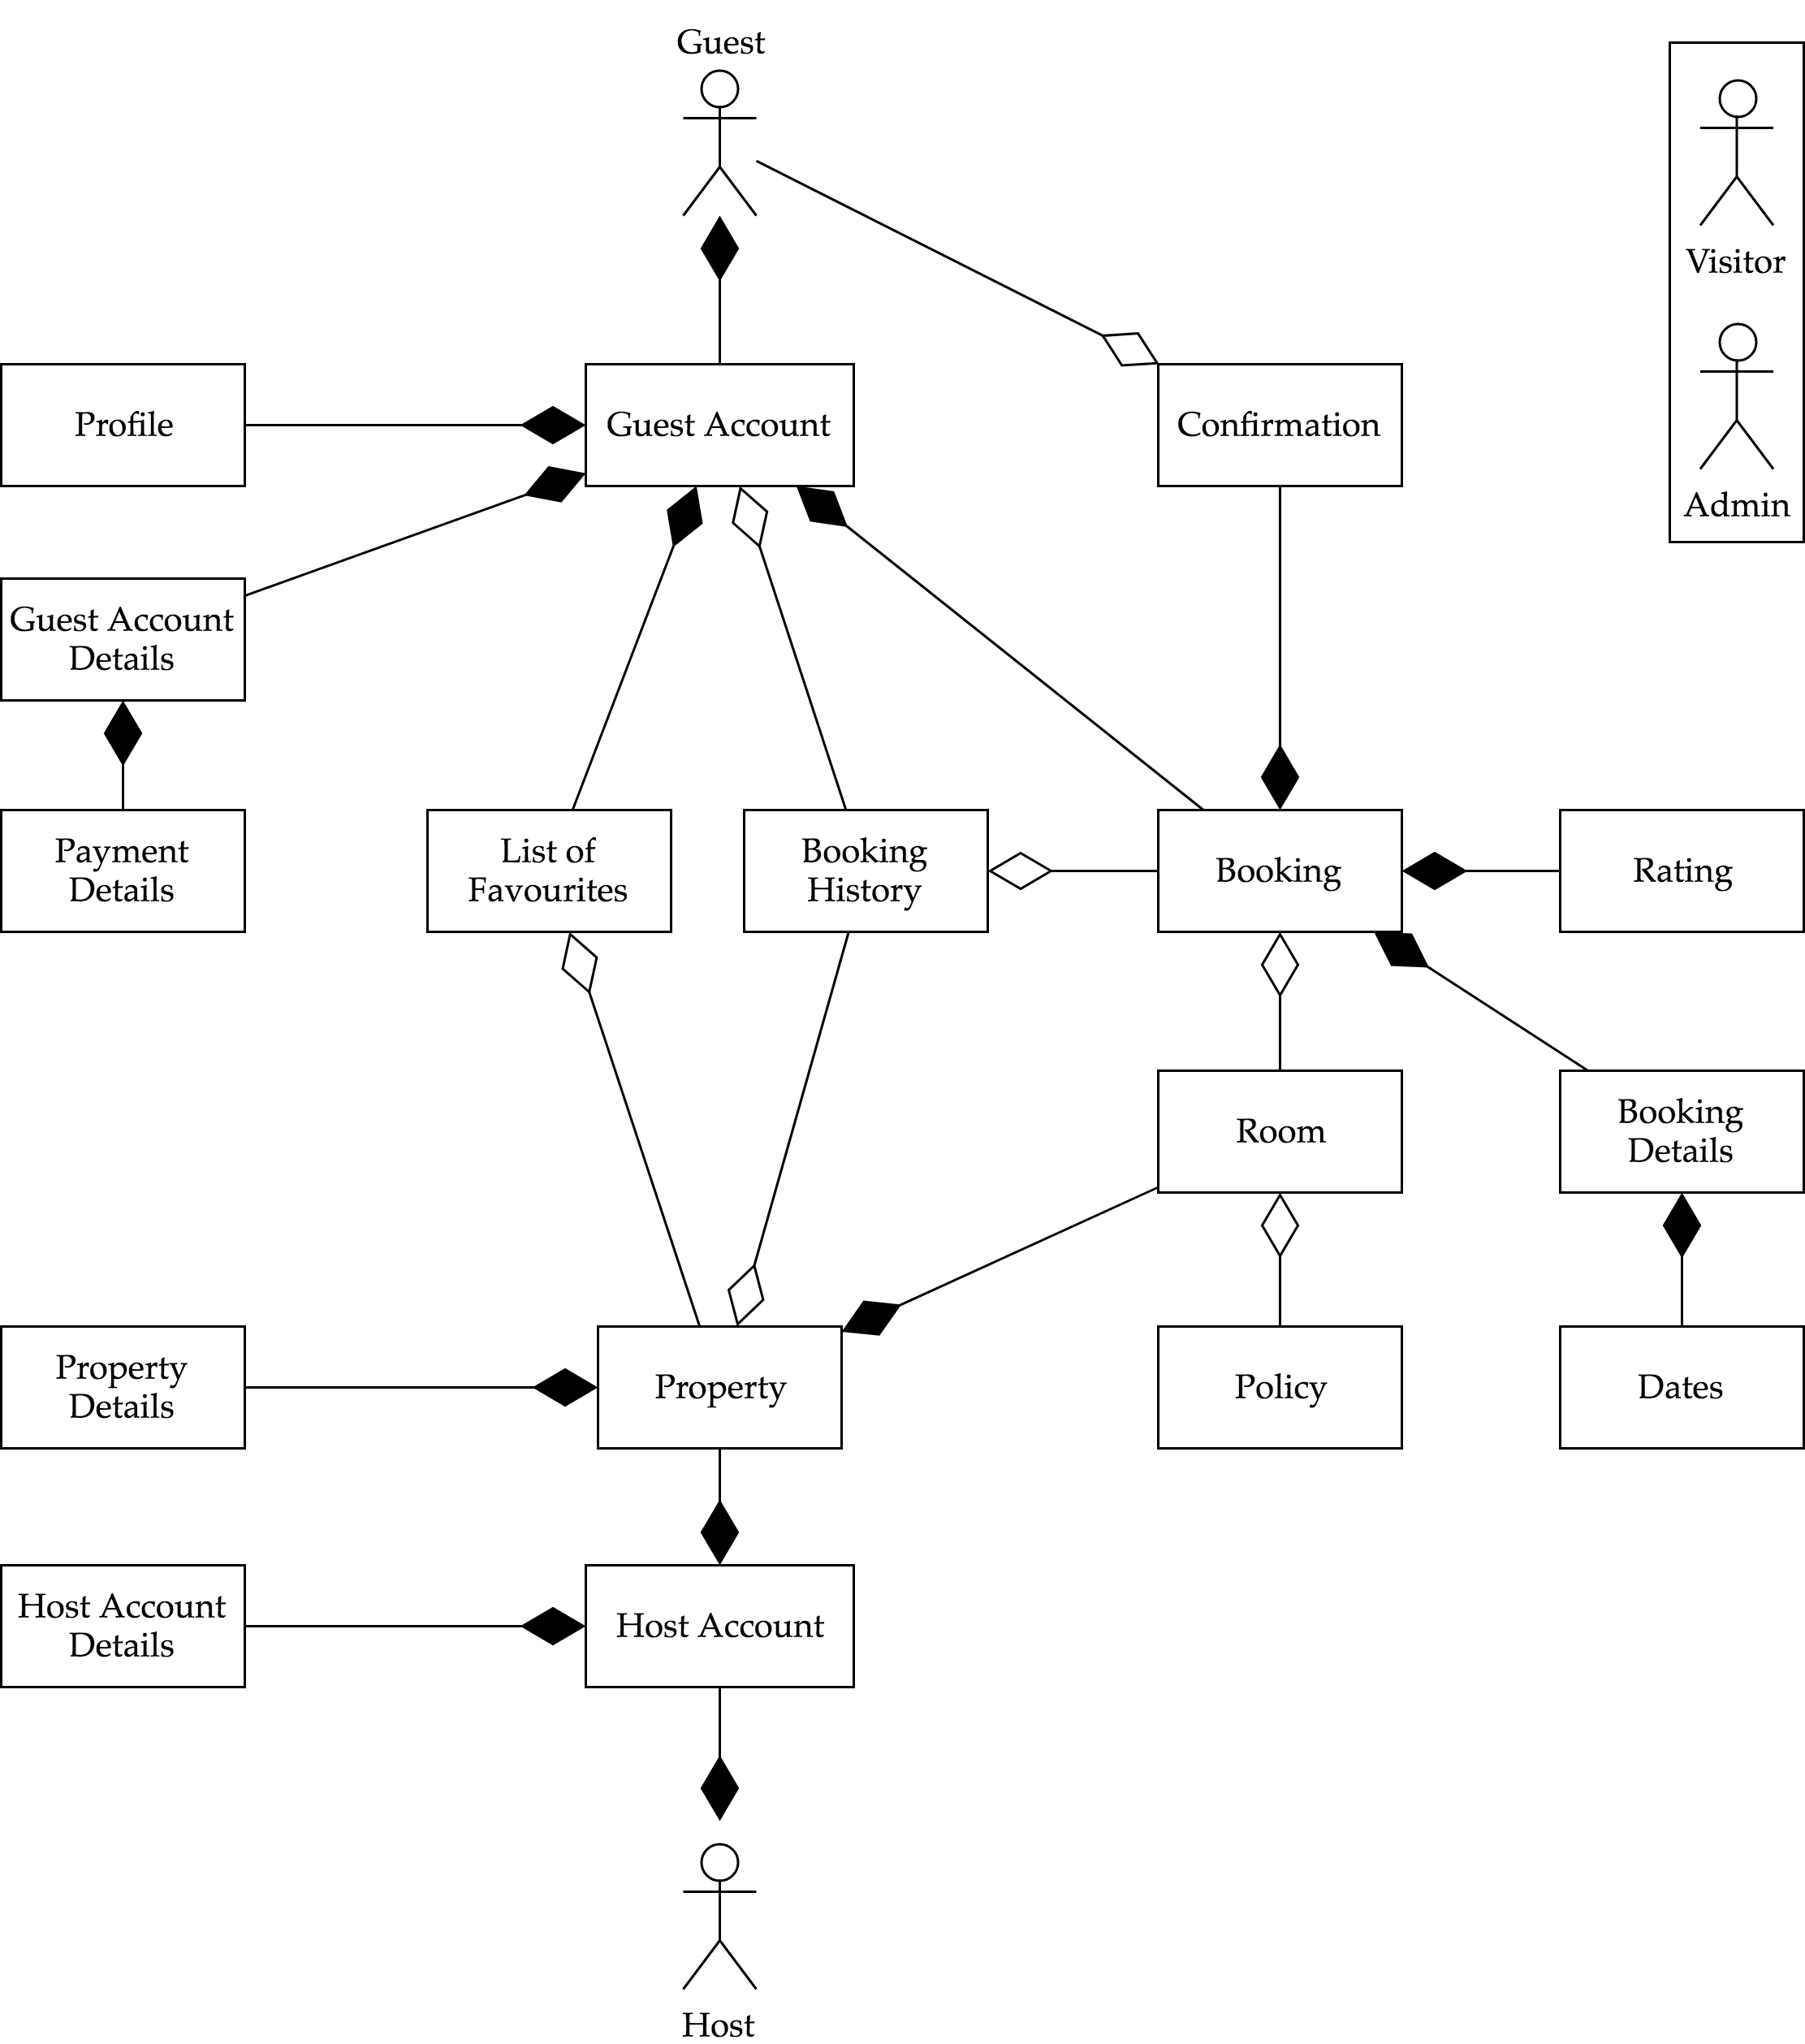
\includegraphics[width=\textwidth]{img/domain_model.png}
    \caption{Domain Model}
    \label{domain_model}
\end{figure}